\documentclass[border=4pt]{standalone}
\usepackage{tikz}
\usetikzlibrary{arrows,arrows.spaced}
\begin{document}
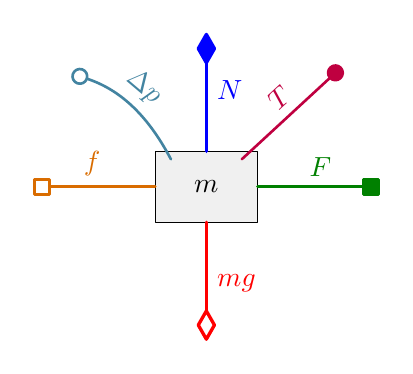
\begin{tikzpicture}[line cap=round,line join=round]
  \draw[fill=gray!12] (-.65,-.45) rectangle (.65,.45);
  \node at (0,0) {$m$};

  \draw[blue,line width=1.2pt,-{spaced diamond}]
    (0,.45) -- node[right] {$N$} (0,2.0);
  \draw[red,line width=1.2pt,-{spaced open diamond}]
    (0,-.45) -- node[right] {$mg$} (0,-2.0);
  \draw[green!50!black,line width=1.1pt,-{spaced square}]
    (.65,0) -- node[above] {$F$} (2.25,0);
  \draw[orange!85!black,line width=1.1pt,-{spaced open square}]
    (-.65,0) -- node[above] {$f$} (-2.25,0);
  \draw[purple,line width=.95pt,-{spaced *}]
    (.45,.35) -- node[above,sloped] {$T$} (1.75,1.55);
  \draw[cyan!60!black,line width=.95pt,{spaced o}-]
    (-1.75,1.45) to[bend left=22] node[above,sloped] {$\Delta p$} (-.45,.35);
\end{tikzpicture}
\end{document}
